\documentclass[aspectratio=169,10pt]{beamer}

% 基本パッケージ
\usepackage{amsmath}
\usepackage{amssymb}
\usepackage{bm}
\usepackage{graphicx}
\usepackage{tikz}

% カラーとテーブル用パッケージ
\usepackage{xcolor}
\usepackage{booktabs}
\usepackage{multirow}
\usepackage{multicol}
\usepackage{tcolorbox}

% 図とアルゴリズム用パッケージ
\usepackage{tikz}
\usetikzlibrary{shapes.geometric}
\usepackage{algorithm}
\usepackage{algpseudocode}

% LuaTeX-jaの読み込み
\usepackage{luatexja}
\usepackage{luatexja-fontspec}

% フォントの基本設定
\usepackage{unicode-math}

% 数式フォントをセリフ体に設定
\setmathfont{Latin Modern Math}

\renewcommand{\kanjifamilydefault}{\gtdefault} % 漢字をゴシック体に指定
\usetheme[block=fill]{metropolis} % usepackageじゃなくてusethemeだから注意

% Proofブロックの定義
\newenvironment{proofblock}[1][]
{\begin{block}{#1}\vspace{0.5em}}
{\vspace{0.5em}\end{block}}

\newenvironment{outlineblock}[1][]
{\begin{tcolorbox}[colframe=black, colback=white, boxrule=1pt, boxsep=5pt]}
{\end{tcolorbox}}

% カラーの設定
\definecolor{titlecolor}{RGB}{0, 60, 120}
\definecolor{sectioncolor}{RGB}{0, 60, 120}
\definecolor{subsectioncolor}{RGB}{0, 60, 120}
\definecolor{boxcolor}{RGB}{240, 245, 255}
\definecolor{boxborder}{RGB}{200, 220, 240}
\definecolor{codecolor}{RGB}{240, 240, 240}

% beamerの設定
% \usetheme{Madrid}
% \usecolortheme{default}
\setbeamertemplate{navigation symbols}{}
\setbeamertemplate{footline}[frame number]  

\title{\textsc{SFC-RG Joint Lecture} \\ Threat Clarification and Correctness Proofs in Protocol Design}
\author{
    Graduate School of Media and Governance, Keio University\\
    \vspace{0.5em}
    Riku MOCHIZUKI\\
    moz@sfc.keio.ac.jp
}
\date{\today}

\begin{document}

\begin{frame}
\titlepage
\end{frame}


\begin{frame}{Topics and Objectives}
\underline{Topics}
\begin{itemize}
    \item Introduction to protocol design
    \item Introduction to threat models
    \item Introduction to formal proofs of protocol correctness
    \item Introduction to research challenges in distributed systems and digital identity
\end{itemize}

\underline{Objectives}
\begin{itemize}
    \item Understand the principles of protocol design in distributed systems
    \item Understand the approach to correctness guarantees in protocol design
    \item Understand how to structure academic papers about protocols and what aspects need to be clarified
\end{itemize}
\end{frame}

\begin{frame}{What is a Protocol?}
\begin{proofblock}[Definition of Protocol (Oxford Dictionary)]
A set of rules governing the exchange or transmission of data between entities.
\end{proofblock}

% Definition of entity
\textbf{Entity}: Refers to individual participants (users, devices) in a protocol.



\begin{proofblock}[Definition of Algorithm (Oxford Dictionary)]
A set of instructions for performing a task or solving a problem.
\end{proofblock}

While algorithms focus on computational procedures, protocols emphasize interactions between participants.
\footnote{Protocols are often explained as conversing using common rules like English or Japanese, which represents interaction rules.
The term ``Japanese algorithm'' is not common because algorithms represent computational procedures rather than interactions.}
Common protocol examples: HTTP, SMTP, TLS/SSL, SSH, OAuth, Paxos, Raft

\end{frame}

\begin{frame}{How to Design Correct Protocols}
This lecture does not cover protocol design methodologies.

\begin{outlineblock}[]
    This lecture focuses on how to explain and demonstrate the correctness of protocols you design in your domain
\end{outlineblock}

To demonstrate protocol correctness, the following aspects must be clarified:
\begin{itemize}
    \item Which entities participate in the protocol
    \item What information exchanges occur between entities
    \item What conditions must be satisfied for the protocol to be achieved the goal
    \item \textbf{What behaviors each entity might exhibit}
    \item \textbf{How to determine whether the protocol is correct\footnote{Satisfying both Safety (bad things don't happen) and Liveness (good things eventually happen) properties} given these entity behaviors}
\end{itemize}

\end{frame}


\begin{frame}{Adversaries and Threat Models}
In protocol design, \underline{clearly defining assumptions about entity capabilities and behaviors} is crucial when considering what behaviors to allow.

\begin{proofblock}[Adversary (Oxford Dictionary)]
An adversary refers to an attacker, typically with malicious intent, who undertakes actions against a system or protocol
\end{proofblock}

In protocol design, an adversary can control entities participating in the protocol, modifying or monitoring their operations.

\vspace{0.5em}
\begin{proofblock}[Threat Model]
A threat model formalizes assumptions about adversary capabilities and behaviors.
\end{proofblock}

\end{frame}

\begin{frame}{Adversaries and Threat Models}

Adversaries control honest entities and introduce corrupted entities into the protocol.
% Adversaries interact with entities using queries like "Send," "Reveal," and "Corrupt"

\begin{figure}
    \centering
    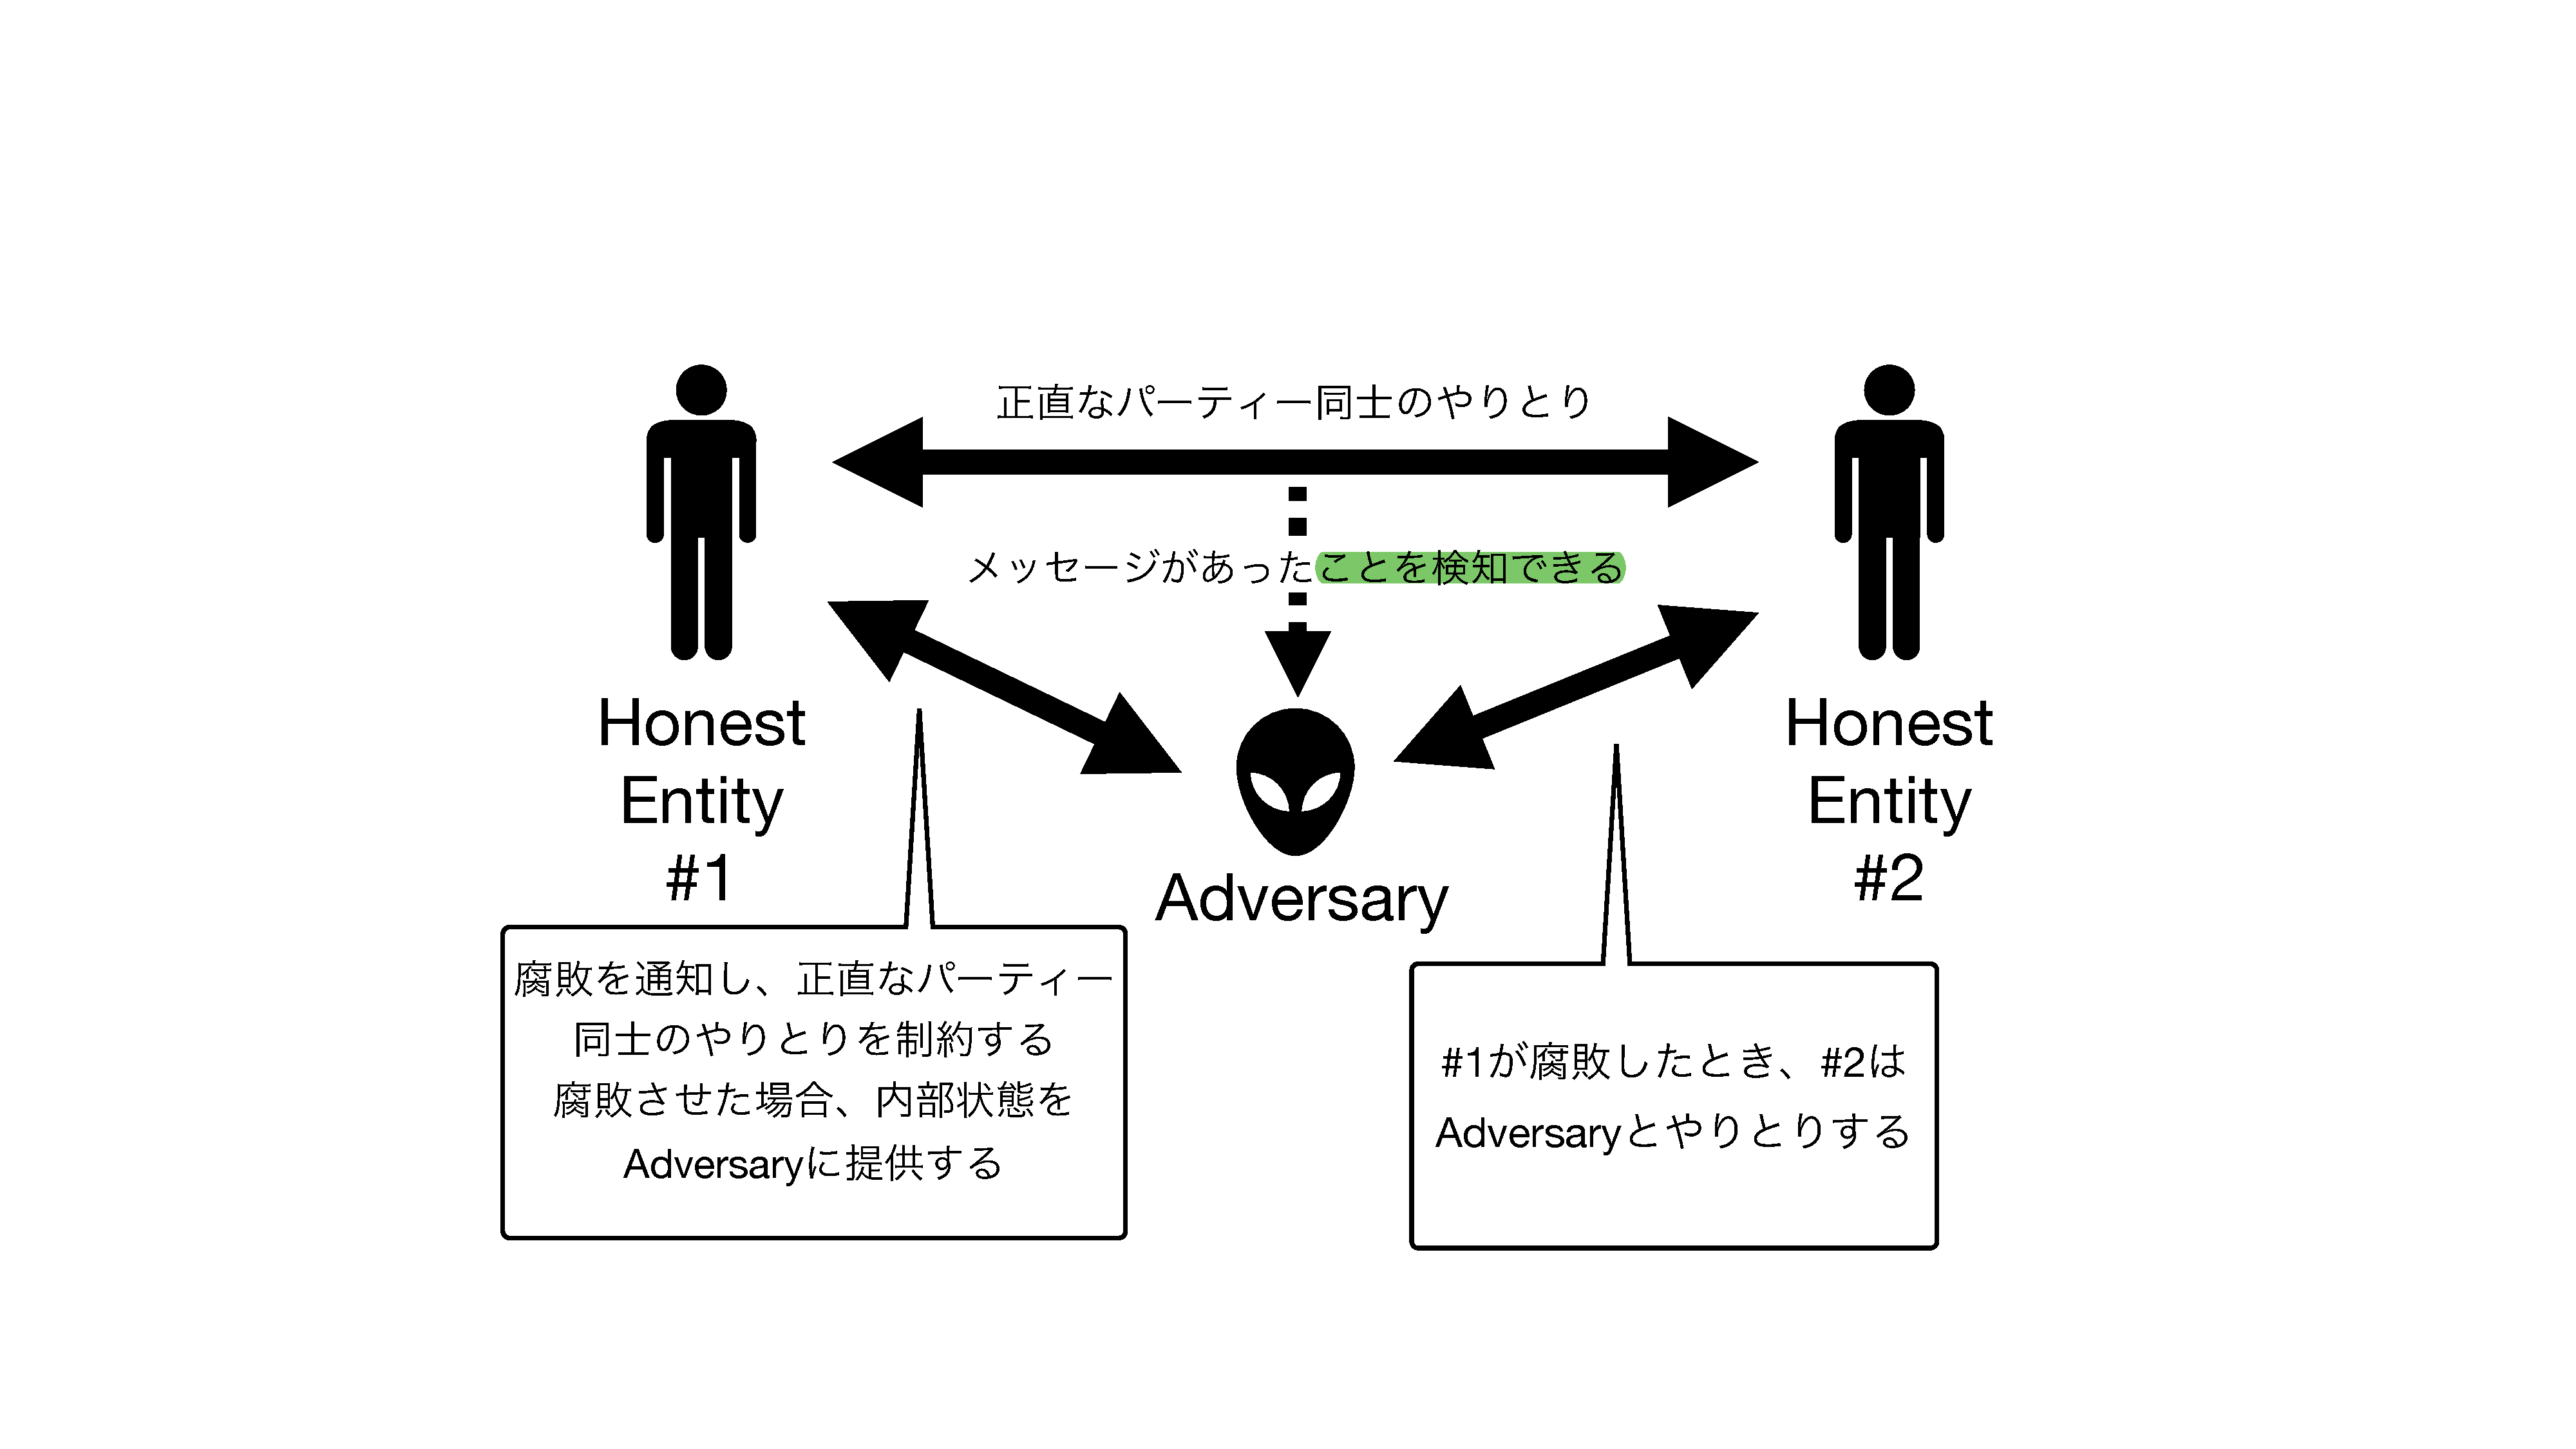
\includegraphics[width=0.5\textwidth]{figs/interaction-adversary.pdf}
    \caption{Relationship between adversaries and entities. Adversaries can introduce corrupted entities into the protocol by intercepting messages from honest entities or directly controlling entities. (Note that entities do not become corrupted directly!)}
    \label{fig:interaction-adversary}
\end{figure}

\end{frame}

\begin{frame}{Components of Threat Models}
Threat models consist of \underline{5 key components}:

\vspace{0.5em}

\begin{enumerate}
    \item \textbf{Corruption Model. }Behavior patterns of entities controlled by the adversary
    \item \textbf{Computational Power. }Constraints on computational resources available to the adversary
    \item \textbf{Adaptivity. }Timing and methods by which the adversary corrupts entities
    \item \textbf{Visibility. }Range of information observable by the adversary
    \item \textbf{Mobility. }Patterns of entity corruption and recovery by the adversary
\end{enumerate}

\vspace{0.5em}

\begin{outlineblock}[]
Different combinations of these components define \underline{different threat models}.
The selection of components depends on the protocol's purpose and the environments in which it may be executed.
\end{outlineblock}
\end{frame}

\begin{frame}{Corruption Models}
Corruption models define how adversaries can control entities.

\vspace{0.5em}

\begin{itemize}
    \item \textbf{Passive. }Follows the protocol completely while accumulating and utilizing all observed information. Cannot deviate from protocol specifications.\footnote{For example, a bank employee who correctly processes customer transaction data while secretly recording and using that data for personal purposes.}\footnote{Also known as Honest-but-Curious or Semi-Honest model.}
    
    \item \textbf{Crash. }Can stop responding at any time but operates according to the protocol outside of downtime.
    
    \item \textbf{Omission. }Entities can arbitrarily delete or ignore received messages but cannot modify the content of messages they send.
    
    \item \textbf{Byzantine. }Entities can arbitrarily deviate from protocol specifications.
\end{itemize}

\vspace{0.5em}

\begin{outlineblock}[]
Each model encompasses the previous models: $\text{Byzantine} \supset \text{Omission} \supset \text{Crash} \supset \text{Passive}$
\end{outlineblock}

\end{frame}

\begin{frame}{Adaptivity Models}
Adaptivity models define when and how adversaries corrupt participants:

\vspace{0.5em}

\begin{itemize}
    \item \textbf{Static}: Adversaries select entities to corrupt before protocol execution and cannot change their selection during execution.
    
    \item \textbf{Adaptive}: Adversaries can dynamically select entities to corrupt during protocol execution.
\end{itemize}

\vspace{0.5em}

\begin{outlineblock}[]
Consider the Adaptive model when there are few entities, many communication phases in the protocol, or long protocol execution times.
For example, key exchange models typically consider the Static model.
Consensus algorithms typically consider the Adaptive model.
\end{outlineblock}
\end{frame}


\begin{frame}{Visibility Models}
Visibility models define the extent to which adversaries can observe messages and internal states.

\begin{itemize}
    \item \textbf{Full Information. }Adversaries can completely observe all message contents and internal states (execution variables) of each entity
    
    \item \textbf{Private Channels.} Communication content between honest entities is completely secret; adversaries can know that messages are being sent and received but cannot see their contents. Internal states of honest entities are also hidden from adversaries.
    
    \item \textbf{Erasure Model. }Extends Private Channels by adding the constraint that adversaries cannot observe or recover data erased before an entity becomes corrupted.
    
    \item \textbf{Oblivious.} Message header information (sender, recipient, length) is observable by adversaries, but message content (payload) is completely hidden. The existence of communication and its metadata are exposed, but the content is protected.\footnote{This concept is used in specific encrypted communication protocols and anonymous communication systems.}
\end{itemize}

% \begin{outlineblock}[]
%     Cryptographic protocols often consider the Private Channels model to guarantee confidentiality (information intended to be kept secret).
% \end{outlineblock}

\end{frame}

\begin{frame}{Computational Power Models}
Computational power models define limitations on adversaries' computational resources:


\begin{itemize}
    \item \textbf{Unbounded. }Adversaries with unlimited computational resources. Theoretically capable of breaking all cryptography.\\
    
    \item \textbf{Polynomially Bounded. }Adversaries limited to polynomial-time computation\footnote{
    When solving a problem, the computational complexity can be expressed as order $O(n^c)$ where $n, c \in \mathbb{Z}$.\\
    Examples include the difficulty of discrete logarithm problems and integer factorization problems.\\
    Generally, Probabilistic Polynomial Time (PPT) refers to algorithms that use randomness and always terminate within polynomial time $\lambda^c$ relative to the security parameter $\lambda \in \mathbb{Z}$ (e.g., key length)}
    
    \item \textbf{Fine-grained. }Adversaries with specific computational limitations.\\
    For example, models with limitations on hash computations per second (Hashrate)
\end{itemize}

\vspace{0.5em}

\begin{outlineblock}[]
The focus is on the adversary's computational power, not the entities' computational power.
Adversaries can observe entity messages and internal states according to the Visibility Model. This model defines what computational resources adversaries can use to utilize that information.
\end{outlineblock}
\end{frame}


\begin{frame}{Mobility Models}
Mobility models define patterns of entity corruption and recovery by adversaries:

\vspace{0.5em}

\begin{itemize}
    \item \textbf{Fixed. }Once corrupted, entities remain corrupted throughout protocol execution and cannot recover
    
    \item \textbf{Mobile. }Adversaries can dynamically corrupt and recover entities. However, there is an upper limit on the total number of corrupted entities at any given time\footnote{Be careful not to confuse this with the Adaptive model in Adaptivity Models. Adaptive refers to the ability of adversaries to choose when to corrupt entities. Mobility considers whether corrupted entities can recover and become honest entities again under those conditions.}
\end{itemize}

\vspace{0.5em}

\begin{outlineblock}[]
From the perspective of IoT, mobile devices, and long-term system operation, the Mobile model is generally considered.
\end{outlineblock}
\end{frame}

\begin{frame}{Importance of Appropriate Assumptions}
In security protocol research, clarifying assumptions is extremely important.

\vspace{0.5em}

\begin{itemize}
    \item If assumptions are too weak: Protocols may be vulnerable to realistic attacks
    \item If assumptions are too strong: Design and implementation may become complex, potentially reducing performance and practicality
\end{itemize}

\vspace{0.5em}

Value of explicit assumptions:
\begin{itemize}
    \item Enables accurate understanding of \underline{protocol correctness}
    \item Allows fair comparison of different protocols using the same criteria
\end{itemize}

\vspace{0.5em}

\begin{outlineblock}[]
In actual system design, selecting appropriate assumptions (threat models) based on specific uses and potential risks is important.
\end{outlineblock}
\end{frame}

\begin{frame}{Example: Practical Byzantine Fault Tolerance (PBFT)}
\begin{proofblock}[PBFT]
\begin{itemize}
    \item PBFT is a replication protocol that \textcolor{red}{tolerates Byzantine faults} while achieving linearizability\footnote{Linearizable replication means all replicas process client requests in the same order, and changes are always reflected within the write request session. Each replicated data is assigned a sequence number and processed according to this sequence number.}\footnote{In Turing-complete state machines, replicated data is viewed as operations (state transition functions). When operations $f$ and $g$ exist, generally $f \circ g \neq g \circ f$, so execution order is important.}
    \item This holds only when $n \geq 3f+1$ (where $f$ is the number of adversaries and $n$ is the total number of replicas).
\end{itemize}
\end{proofblock}

The PBFT protocol was the first to demonstrate achieving linearizability in the partial synchrony model.
Even 20 years after its introduction, PBFT remains widely used.


\end{frame}

\begin{frame}{PBFT Protocol Details (1)}
Main phases of PBFT:
\vspace{0.5em}
\begin{enumerate}
    \item \textbf{Pre-prepare}: Primary (leader) $p$ assigns sequence number $s$ to client request $r$ and sends $\langle \text{PRE-PREPARE}, s, r \rangle$ message to other replicas
    
    \item \textbf{Prepare}: Replicas agree on request order and send $\langle \text{PREPARE}, s, r \rangle$ message to all replicas
    
    \item \textbf{Commit}: Replicas that receive at least $2f+1$ PREPARE messages send $\langle \text{COMMIT}, s, r \rangle$ message, committing to execution
    
    \item \textbf{Reply}: Replicas that receive $2f+1$ COMMIT messages execute the request and send results to the client
\end{enumerate}
\end{frame}


\begin{frame}{PBFT Protocol Details (2)}

\begin{figure}[h]
    \centering
    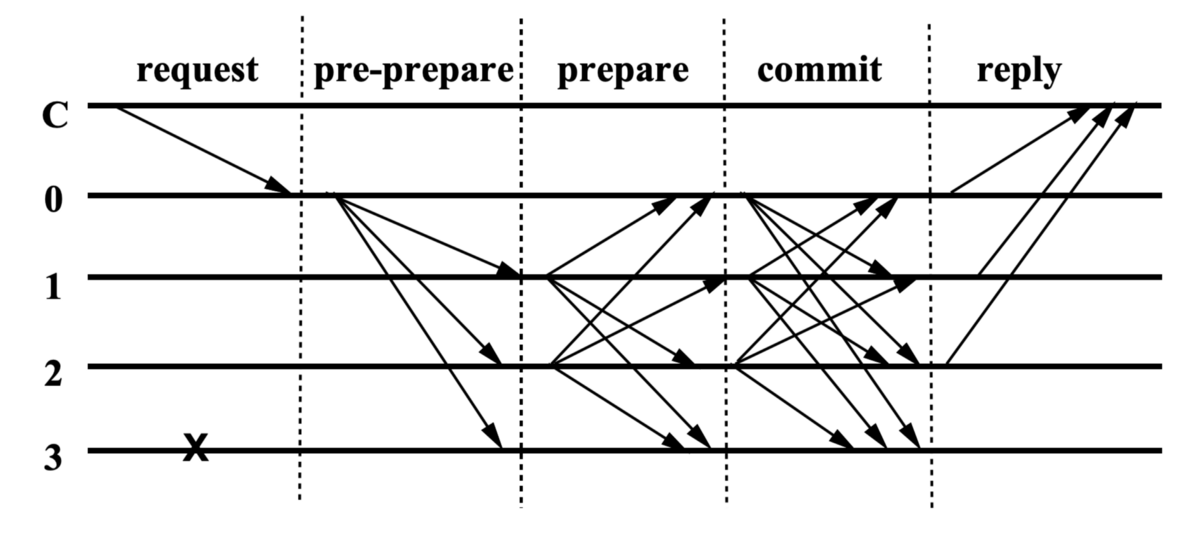
\includegraphics[width=0.9\textwidth]{figs/pbft-sequence.png}
    \caption{PBFT sequential diagram}
    \label{fig:pbft_protocol}
\end{figure}

\end{frame}

\begin{frame}{PBFT Threat Model}
Let's consider the PBFT threat model.
\begin{proofblock}[PBFT Threat Model $\Lambda_{PBFT}$]
\begin{itemize}
    \item \textbf{Corruption}: \textcolor{red}{Byzantine} - Replicas can behave arbitrarily, such as sending different messages to different replicas
    \item \textbf{Adaptivity}: Adaptive - Adversaries can dynamically corrupt different replicas in each phase of the protocol
    \item \textbf{Computational Power}: Polynomially Bounded - Limited to polynomial-time computation
    \item \textbf{Visibility}: Private channels - Communication content between honest replicas is secret, and internal states are not visible to adversaries
    \item \textbf{Mobility}: Fixed - Once corrupted, replicas remain corrupted throughout protocol execution and cannot recover
\end{itemize}
\end{proofblock}
\end{frame}

\begin{frame}{PBFT Correctness Guarantees}

\begin{proofblock}[PBFT Correctness Guarantees]
When $n \geq 3f + 1$ (where $f$ is the number of corrupted nodes and $n$ is the total number of replicas):
\begin{itemize}
    \item \textbf{\textcolor{red}{Safety}}: Honest replicas never commit different values for the same sequence number
    \item \textbf{\textcolor{red}{Liveness}}: All client requests are eventually processed and responses are returned
\end{itemize}

\vspace{0.5em}

If we can prove that PBFT satisfies both Safety and Liveness, then PBFT can be considered correct.
\end{proofblock}
In other words, if we can prove that PBFT satisfies Safety and Liveness regardless of what attacks adversaries perform within the threat model $\Lambda_{PBFT}$, then PBFT can be considered correct.

\vspace{0.5em}


\textbf{Question}: Why is Safety satisfied when $n \geq 3f + 1$? Let's explain why PBFT is secure!
\end{frame}

\begin{frame}{PBFT Safety Proof}
Assumption: Two different values $v$ and $v'$ are committed with the same sequence number $s$.

\begin{lemma}
For each value to be committed, COMMIT messages from at least $2f+1$ replicas are required. (Out of $3f+1$ total replicas, at most $f$ can be corrupted)
\end{lemma}

\begin{itemize}
\item \small Value $v$ requires COMMIT messages from at least $2f+1$ replicas in set $\mathcal{P}$
\item \small Similarly, value $v'$ requires COMMIT messages from at least $2f+1$ replicas in set $\mathcal{Q}$
\item \small $| \mathcal{P} \cap \mathcal{Q} | \geq 2f+1 + 2f+1 - n \geq 4f+2 - (3f+1) = f+1$
\item \small The intersection $\mathcal{P} \cap \mathcal{Q}$ contains at least $f+1$ replicas, and since the system has at most $f$ Byzantine replicas, \underline{at least $1$ honest replica must have sent COMMIT messages for both values $v$ and $v'$}
\item \small However, honest replicas never send COMMIT messages for different values with the same sequence number, creating a contradiction
\item \small Therefore, the assumption is false
\end{itemize}
\end{frame}

\begin{frame}{Correctness Proofs for Complex Protocols}
  In practice, simple protocols like PBFT are rare, and composite protocols that combine existing protocols as components are common.

  \begin{itemize}
    \item Application layer protocols are often built on existing replication layers (e.g., PBFT)
          \footnote{Example: Building a timestamp mechanism on top of PBFT. Related to kekeho's GP2.}
  \end{itemize}

  \begin{proofblock}[Hybrid Protocol]
    A hybrid protocol obtained by combining $n$ protocols $\pi_1,\dots,\pi_n$ is denoted as $\pi[\pi_1,\dots,\pi_n]$.
    
  \end{proofblock}

  \textbf{Motivation}: How to demonstrate the correctness of composite protocol $\pi[\pi_1,\dots,\pi_n]$?
  \begin{itemize}
    \item Can we analyze each component individually to prove the correctness of the whole?
    \item How to guarantee correctness in any environment?
  \end{itemize}
\end{frame}

\begin{frame}{Universal Composability Framework}
Using the UC Framework, the correctness of complex protocols can be demonstrated based on the completeness guarantees of simple components.
In other words, to prove that a composite protocol $\pi[\pi_1,\dots,\pi_n]$ is correct, we need to prove the correctness of each component $\pi_1,\dots,\pi_n$ and show that they are combined appropriately.

  \begin{proofblock}[Definition of Ideal Functionality $\mathcal{F}$]
    An ideal functionality $\mathcal{F}$ receives inputs from entities, computes $f$, and returns outputs to each entity.
    In other words, it defines the protocol interface and defines a mapping $f$ that returns outputs for any input.\footnote{This can be considered as an indestructible (i.e., the interface or mapping $f$ cannot be modified) trusted entity.}
  \end{proofblock}

  \begin{proofblock}[Definition of Protocol $\pi$]
    A protocol $\pi$ is an actual program, a procedure executed between multiple entities (concrete implementation of the protocol).
    It is designed to realize the ideal functionality $\mathcal{F}$.
  \end{proofblock}
\end{frame}

\begin{frame}{Ideal/Real World Paradigm}
    UC has two worlds for executing ideal functionality $\mathcal{F}$ and protocol $\pi$:

    \begin{proofblock}[Ideal World]
    \begin{itemize}
      \item The ideal functionality $\mathcal{F}$ performs computations, and the adversary behaves as a simulator $Sim$.
      \item Dummy entities send inputs to $\mathcal{F}$ and return outputs from $\mathcal{F}$ to the environment $\mathcal{Z}$.
      \item The simulator $Sim$ mimics the behavior of the real-world adversary through the interface with the ideal functionality $\mathcal{F}$ and returns the results to the environment.
    \end{itemize}
  \end{proofblock}
\end{frame}


\begin{frame}{Ideal/Real World Paradigm}
    UC has two worlds for executing ideal functionality $\mathcal{F}$ and protocol $\pi$:

  \begin{proofblock}[Real World]
    \begin{itemize}
      \item The real world consists of the actual protocol $\pi$, its participating entities, and the adversary $\mathcal{A}$.
      \item Entities communicate with each other according to protocol $\pi$ while advancing the computation.
      \item The adversary $\mathcal{A}$ controls corrupted entities, and all internal states and actions are controlled by $\mathcal{A}$.
      \item The environment $\mathcal{Z}$ provides inputs to entities and the adversary and collects all outputs.
    \end{itemize}
  \end{proofblock}
\end{frame}

\begin{frame}{Ideal/Real World Paradigm}
  \begin{outlineblock}{}
    In other words... each world can be interpreted as follows:
    \begin{itemize}
        \item The ideal world can be considered as "a world where a trusted entity $\mathcal{F}$ performs all processing."
        \item The real world can be considered as "a world where entities communicate with each other to perform processing because there are no trusted entities."
        \item Therefore, a protocol being correct means that the protocol $\pi$ executed by entities in the real world is indistinguishable from the ideal functionality $\mathcal{F}$ executed in the ideal world.\footnote{More precisely, it is indistinguishable with negligible probability. This is because UC holds only against probabilistic polynomial-time (PPT) adversaries. Regarding probabilistic polynomial time, as mentioned earlier, it can be approximated as order $O(n^c)$ in a probabilistic Turing machine.}
    \end{itemize}
  \end{outlineblock}
\end{frame}


\begin{frame}{Environment Entity Operating Ideal and Real Worlds}
    The entity that operates these two worlds is the environment $\mathcal{Z}$.
    \begin{proofblock}[Environment $\mathcal{Z}$]
    \begin{itemize}
      \item The environment $\mathcal{Z}$ abstracts all systems outside the protocol (such as other protocols).
      \item In the ideal world, $\mathcal{Z}$ sends protocol inputs to dummy entities and receives their outputs and outputs from the simulator $Sim$.\footnote{More precisely, the environment does not communicate directly with $\mathcal{F}$ but interacts indirectly through dummy entities}
      \item In the real world, $\mathcal{Z}$ sends inputs to entities executing the protocol and receives their outputs and outputs from the adversary $\mathcal{A}$.
      \item $\mathcal{Z}$ tries to distinguish whether it is interacting with the ideal world or the real world.\footnote{In other words, $\mathcal{Z}$ tries to find differences between the behavior of the actual protocol and entities in the real world and the behavior of the ideal functionality and dummy entities in the ideal world.}
    \end{itemize}
  \end{proofblock}
\end{frame}

\begin{frame}{Comparison of Ideal and Real Worlds}

    \begin{figure}[h]
        \centering
        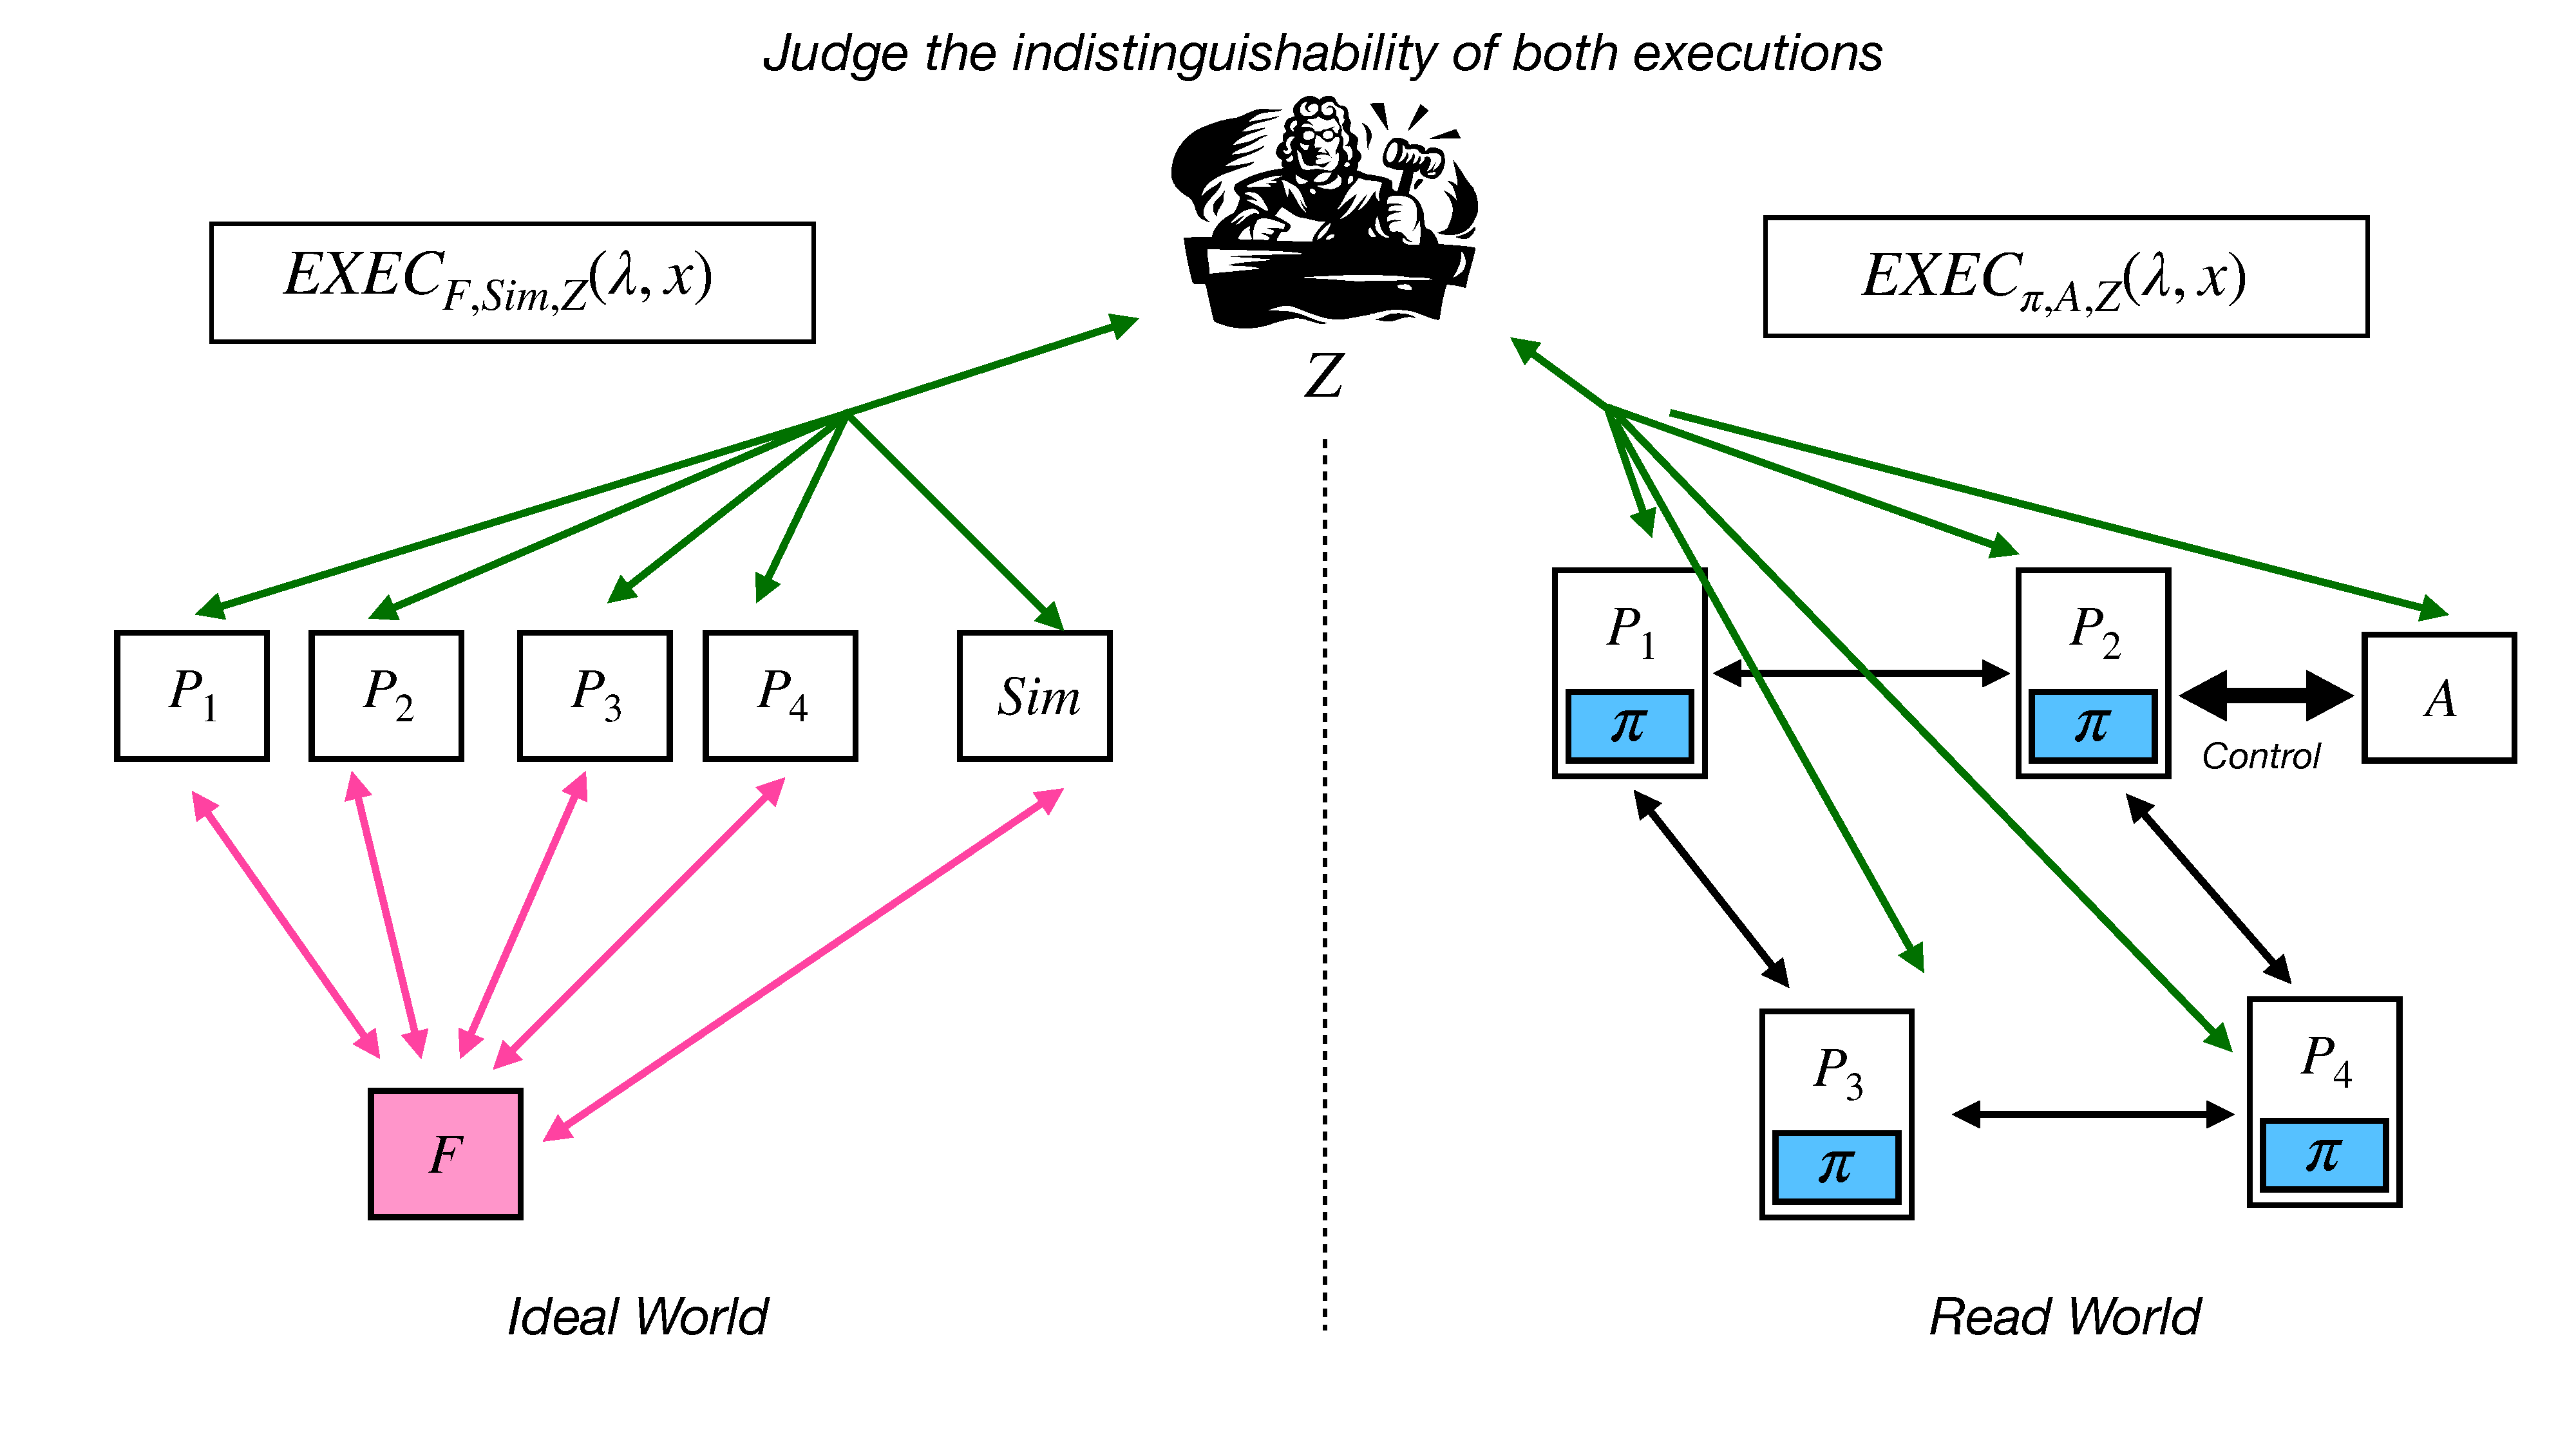
\includegraphics[width=0.65\textwidth]{figs/uc.pdf}
        \caption{Interaction between ideal and real worlds. In the ideal world, each dummy party $P_i$ communicates directly with the ideal functionality $\mathcal{F}$, while in the real world, entities $P_i$ executing protocol $\pi$ communicate with each other. This perspective allows $\mathcal{F}$ to be considered as a trusted ideal functionality.}
        \label{fig:uc_comparison}
    \end{figure}

\end{frame}

\begin{frame}{Correctness Claims in UC}
  
  \begin{proofblock}[Definition of UC Correctness]
   If the environment $\mathcal{Z}$ tries to find differences between interactions in the real world and the ideal world but cannot distinguish between them, then $\pi$ can be said to correctly realize the ideal functionality $\mathcal{F}$.
   This is called ``$\pi$ UC-realizes $\mathcal{F}$.''

    \medskip
    \small \textbf{Rigorous Definition. }
    \small For security parameter $\lambda \in \mathbb{N}$ and protocol $\pi$, we say that $\pi$ "UC-realizes" the ideal functionality $\mathcal{F}$ when:
    \small For any probabilistic polynomial-time\footnote{UC holds only against probabilistic polynomial-time adversaries} adversary $\mathcal{A}$, there exists a probabilistic polynomial-time algorithm $Sim$ such that for any probabilistic polynomial-time environment $\mathcal{Z}$ and any input $x \in \{0,1\}^*$:
    \[ EXEC_{\mathcal{F},Sim,\mathcal{Z}}(\lambda, x) \approx EXEC_{\pi,\mathcal{A},\mathcal{Z}}(\lambda, x) \]
  \end{proofblock}
\end{frame}

\begin{frame}{Benefits of Using UC for Correctness Proofs}
  \begin{itemize}
    \item \textbf{Modularity. } Complex tasks can be decomposed into smaller protocols, and the correctness of each protocol can be proven independently.
    \item \textbf{Composition Theorem. } If protocol $\pi$ UC-realizes ideal functionality $\mathcal{F}$ and protocol $\rho$ using $\mathcal{F}$ UC-realizes ideal functionality $\mathcal{G}$, then the protocol $\rho^{\mathcal{F} \rightarrow \pi}$ obtained by replacing $\mathcal{F}$ with $\pi$ also UC-realizes $\mathcal{G}$.
  \end{itemize}

  \vspace{1em}

  \begin{outlineblock}{}
    The core of the UC framework is "composability": the correctness of a protocol, once proven, is maintained in any complex environment. This enables the incremental construction and reuse of secure protocols.
  \end{outlineblock}
\end{frame}

\begin{frame}{Protocol Instances and Session Identification}
  In the real world, multiple copies of the same protocol are executed simultaneously by different users.
  A protocol is like a type, and instances of that type are actually executed.
  
  \begin{proofblock}[Protocol Instance]
    An instance of protocol $\pi$ is a specific execution of that protocol, typically distinguished by a unique identifier.
  \end{proofblock}
  
  \begin{itemize}
    \item \textbf{Session Identifier ($sid$)}: A unique identifier that distinguishes each protocol execution
    \item For example... on blockchains, smart contract addresses function as $sid$
  \end{itemize}
  
  \begin{outlineblock}{}
    In the basic UC framework, each protocol instance has its own instance.
    However, this may not be realistic in some cases (e.g., when the same hash function is used in multiple protocols).
  \end{outlineblock}
\end{frame}

\begin{frame}{Generalized Universal Composability (GUC) Framework}
  \begin{proofblock}[What is the GUC Framework]
    An extension of the UC framework that introduces the concept of "global functionalities" shared across multiple protocol instances.
  \end{proofblock}
  
  \begin{proofblock}[Global Functionality]
    \begin{itemize}
      \item Functionality shared across multiple protocol instances
      \item Examples: hash functions, digital signatures, shared ledgers
      \item Maintains consistent internal state across all protocol sessions
    \end{itemize}
  \end{proofblock}

  GUC not only enables parallel execution environments but also eliminates the need to analyze instances individually.
\end{frame}


\begin{frame}{Why Learn These Correctness Proof Methods?}
\begin{outlineblock}
     To write academic papers in formats accepted by the academic community.\footnote{Especially for international journals and top conferences. Top conferences have acceptance rates of 20\% or lower, or CORE rank $A$ or $A^{+}$ conferences}
     Without these methods, papers may be rejected outright even if the protocol design appears good.
\end{outlineblock}

Simply describing protocol specifications and implementations is insufficient\\
``
\textit{Since there is no formal security model, it is hard to verify the formal correctness of the claims. Moreover, the scheme includes many low-level implementation details instead of giving a general description of their scheme.}
''
\\
\small(Excerpt from a review comment received by moz two years ago from CRYPTO'23, a top conference)

\begin{figure}
        \centering
        
\includegraphics[width=0.58\textwidth]{figs/uc-citation.png}
        \caption{Number of citations for the UC framework as of April 30, 2023}
        \label{fig:uc_citation}
\end{figure}
\end{frame}


\begin{frame}{Let's Examine a Paper Published in a Top Conference}
Let's examine a paper titled "FairSwap: How to Fairly Exchange Digital Goods" published in ACM CCS 2020, a top conference.
\begin{outlineblock}{}
    This paper proposes a protocol for exchanging digital data $x$ and $y$ between $\mathcal{A}$ and $\mathcal{B}$.
    The protocol guarantees that either both conditions
    $P: \mathcal{A} \stackrel{x}{\rightarrow} \mathcal{B}$ and 
    $Q: \mathcal{B} \stackrel{y}{\rightarrow}  \mathcal{A}$
    are satisfied, or neither is satisfied.

    \medskip

    The paper defines the ideal functionality $\mathcal{F}_{fe}$ along with the global functionality $\mathcal{L}$ with blockchain capabilities and a random oracle $\mathcal{H}$.
    
\end{outlineblock}

\begin{center}
    \url{https://dl.acm.org/doi/pdf/10.1145/3243734.3243857}
\end{center}

\begin{figure}
        \centering
        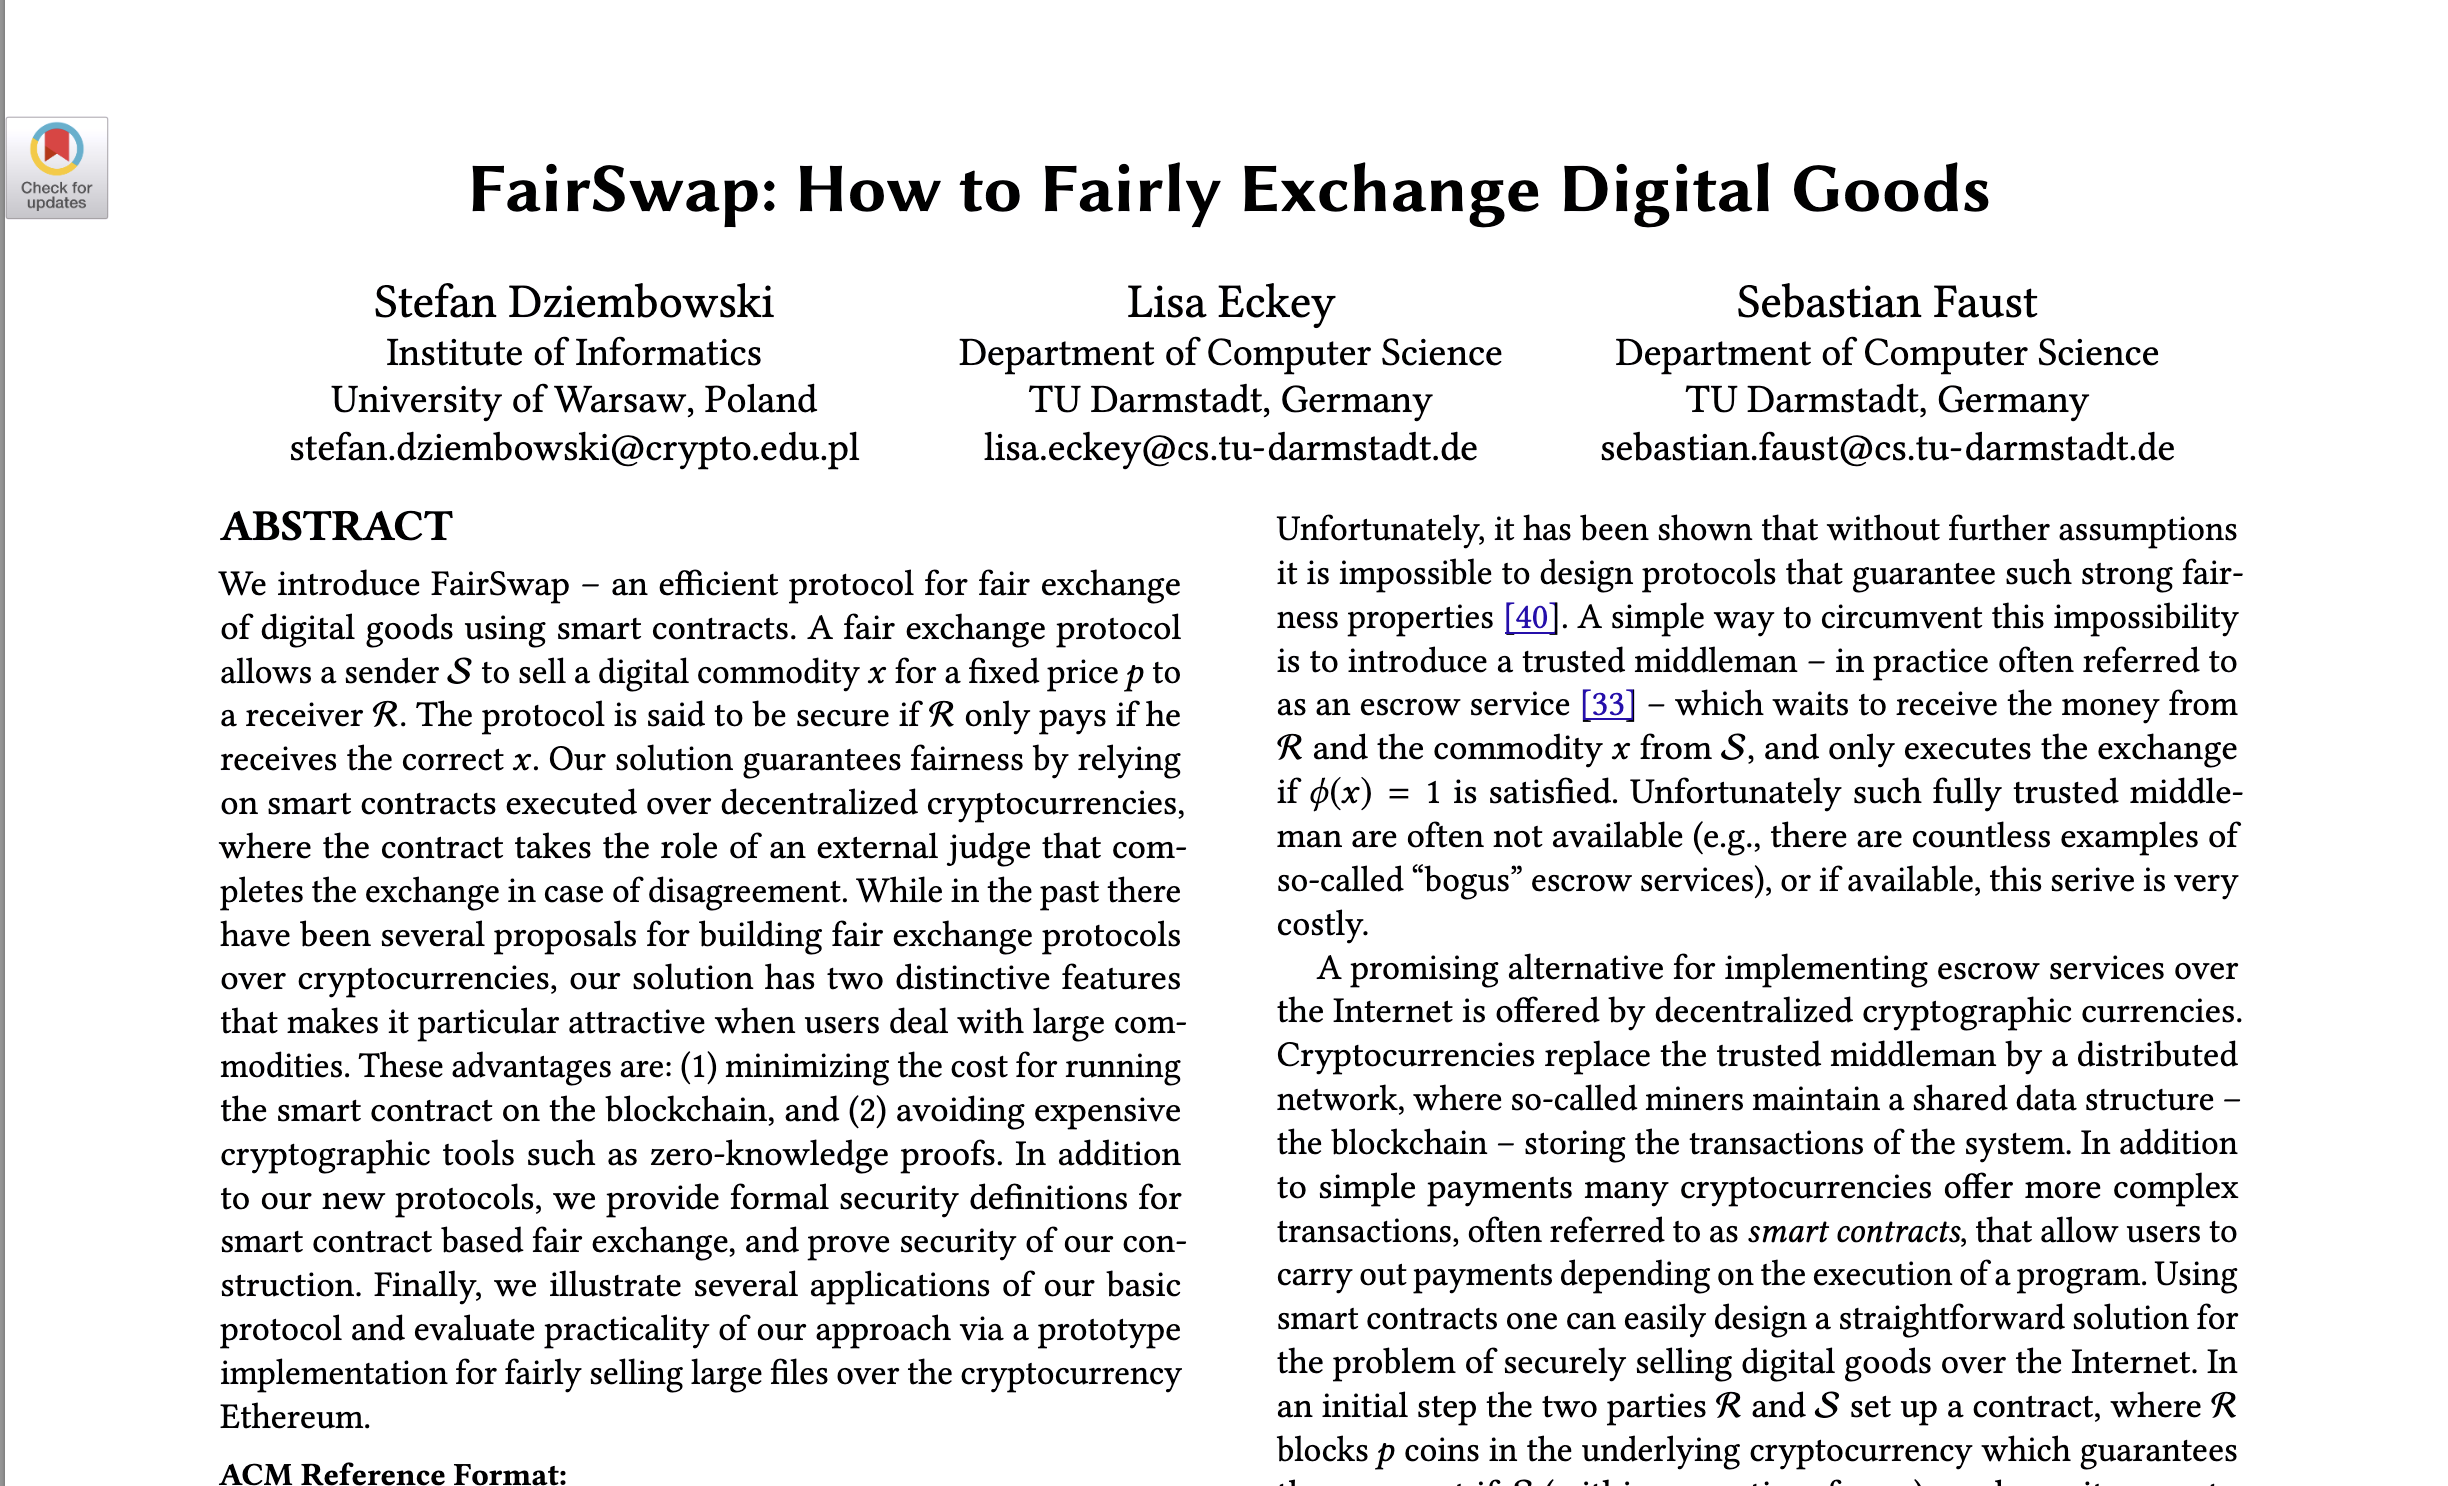
\includegraphics[width=0.58\textwidth]{figs/fairswap.png}
        \caption{Number of citations for the UC framework as of April 30, 2023}
        \label{fig:uc_citation}
\end{figure}
\end{frame}


\begin{frame}{Are These Assumptions Sufficient?}
The assumptions we have used so far are:
\begin{itemize}
    \item \textbf{Network Model}: Asynchronous, synchronous, or partially synchronous (with an upper bound on communication delay)
    \item \textbf{Adversary Model}: How adversaries behave
    \item \textbf{Number of Corrupted Nodes}: Conditions on the number of entities the attacker can control (e.g., $n \geq 3f+1$)
\end{itemize}

\textbf{Question}: Are these the only threats and assumptions to consider when operating in the real world?
\end{frame}

\begin{frame}{Sybil Attack}
With just these assumptions, all protocols are vulnerable to Sybil Attacks.

\begin{proofblock}[Sybil Attack]
An attack where a single entity impersonates multiple entities to gain undue influence in a system.\footnote{One entity plays the roles of two different identities, but other entities cannot determine whether these identities belong to the same entity.}
\end{proofblock}

\begin{outlineblock}[Conditions for Sybil Attack]
    PBFT requires the condition $n \geq 3f+1$, where $n$ is the number of nodes and $f$ is the number of adversaries.
    This implicitly assumes that each replica is uniquely identifiable and message origins are authentic.
    If an adversary can behave as multiple entities, this condition breaks down.\footnote{This allows certain compromises in the Byzantine Corruption Model. Is this acceptable?}
\end{outlineblock}
\end{frame}

\begin{frame}{Digital Signatures}
To verify the authenticity of message origins, messages must be digitally signed and these signatures must be verified.

\begin{proofblock}[Digital Signatures]
    Digital signatures use mathematically related public key (verification key) $pk$ and private key (signing key) $sk$ pairs to verify message origins.
    \begin{itemize}
        \item Signing a message $m$: $\sigma \gets \textsc{Sign}(sk, m)$
        \item Verifying a message $m$ with signature $\sigma$: $\{0, 1\} \gets \textsc{Verify}(pk, m, \sigma)$ where $1$ if $m$ is valid, $0$ otherwise
    \end{itemize}
\end{proofblock}
Specific digital signature schemes include RSA, ECDSA, EdDSA, and Schnorr signatures.
\end{frame}


\begin{frame}{Verifying Message Authenticity}
When entity $\mathcal{P}$ sends a message $m$ to entity $\mathcal{Q}$, 
entity $\mathcal{Q}$ needs to verify that message $m$ was indeed received from $\mathcal{P}$.

\vspace{0.5em}

\begin{itemize}
    \item Entity $\mathcal{P}$ generates a digital signature $\sigma$ for message $m$ using the private key $sk_{\mathcal{P}}$ corresponding to public key $pk_{\mathcal{P}}$.
    \item $\mathcal{P}$ sends $(m, \sigma)$ to $\mathcal{Q}$.
    \item $\mathcal{Q}$ verifies the received $(m, \sigma)$: $\textsc{Verify}(pk_{\mathcal{P}}, m, \sigma) \stackrel{?}{=} 1$
\end{itemize}

\begin{outlineblock}[Assumption Required for Verifying Message Authenticity with Digital Signatures]
    Assumption needed to ensure verification validity: $\mathcal{Q}$ knows $\mathcal{P}$'s public key $pk_{\mathcal{P}}$.
\end{outlineblock}

\textbf{Question}: Is this sufficient to prevent Sybil Attacks?

\end{frame}



\begin{frame}{Cost of Generating Identifiers}
\textbf{Answer}: Insufficient.
The proposition ``Digital signatures can distinguish message origins $\Leftrightarrow$ Entities can be distinguished'' does not necessarily hold.

\begin{outlineblock}
    Digital signatures can distinguish message senders, but verification validity is not guaranteed unless a \underline{one-to-one correspondence} between entities and public keys is assumed.
\end{outlineblock}

\begin{itemize}
    \item A single entity can generate multiple public keys and behave as multiple entities
    \item A Key Management System\footnote{Key Management System (KMS) guarantees one-to-one correspondence between entities and public keys. Public Key Infrastructure (PKI) is a type of Key Management System.} is necessary to ensure one-to-one correspondence between entities and public keys. KMS verifies this correspondence\footnote{Verification involves two aspects. First, verifying that an entity claiming to be a specific identity is indeed that identity. Second, defining a mapping between entities and public keys, and confirming this relationship is bijective. After confirmation, KMS issues a signature (=certificate) indicating the binding is valid. Users can substitute this verification with signature verification by trusting the KMS.}
\end{itemize}
\end{frame}

\begin{frame}{Problems with KMS}
However, KMS has the following issues:
\begin{itemize}
    \item Allowing certification authorities = assuming the existence of trusted third parties
    \item Creates single points of failure and scalability problems
\end{itemize}
Other approaches like \textbf{Proof-of-Work} require computational resources for creating new identifiers.

\begin{outlineblock}
    \begin{itemize}
        \item When examining protocols (with Byzantine Fault Tolerance) in the context of distributed systems, bottlenecks exist (implicit, non-trivial assumptions) that prevent maximizing the appeal and effectiveness of distributed systems. These are not always documented in academic papers.
    \end{itemize}
\end{outlineblock}

\end{frame}


\begin{frame}{One more thing}
How to find impactful problems?
\begin{outlineblock}
    \begin{itemize}
        \item Having operational experience expands the options for interpreting protocols discussed in theory.
        \item This means changing the situation in which a protocol operates (assumptions supporting the logic of the proposed protocol\footnote{For example, adversary models, network, and timing models}) based on insights gained from operations, and determining whether bottlenecks can be ignored or not.
        \item I believe such exploration contributes to impactful and clear problem statements.
    \end{itemize}
\end{outlineblock}
This lecture provided a theoretical perspective, but hearing operational viewpoints from other kGs may bring new interpretations to your research (field).
I hope this general lecture becomes a forum where we organically generate, share, and enhance such interpretations together.
\end{frame}

% ・・・・・・・・・・



\end{document}